\documentclass{article}

\usepackage{polski}
\usepackage[utf8]{inputenc}

\usepackage{fancyhdr} % Required for custom headers
\usepackage{lastpage} % Required to determine the last page for the footer
\usepackage{extramarks} % Required for headers and footers
\usepackage[usenames,dvipsnames]{color} % Required for custom colors
\usepackage{graphicx} % Required to insert images
\usepackage{listings} % Required for insertion of code
\usepackage{courier} % Required for the courier font
\usepackage{lipsum} % Used for inserting dummy 'Lorem ipsum' text into the template\
\usepackage{amsfonts}
\usepackage{amsthm}
\usepackage{hyperref}
\usepackage{tikz}
\usepackage{amsmath}
\usepackage{pdfpages}
\usepackage{mathtools}


\newtheorem{thm}{Twierdzenie}
\newtheorem{remark}{Uwaga}
\newtheorem{lemat}{Lemat}


\newenvironment{prooff}{\paragraph{Dowód:}}{\hfill$\square$}
\newenvironment{rozw}{\paragraph{Rozwiazanie:}}{\hfill}

% Margins
\topmargin=-0.45in
\evensidemargin=0in
\oddsidemargin=0in
\textwidth=6.5in
\textheight=9.0in
\headsep=0.25in

\linespread{1.1} % Line spacing

% Set up the header and footer
\pagestyle{fancy}
\lhead{\hmwkAuthorName} % Top left header
\chead{\hmwkClass\ (\hmwkClassInstructor\ \hmwkClassTime): \hmwkTitle} % Top center head
\rhead{\firstxmark} % Top right header
\lfoot{\lastxmark} % Bottom left footer
\cfoot{} % Bottom center footer
\rfoot{Page\ \thepage\ of\ \protect\pageref{LastPage}} % Bottom right footer
\renewcommand\headrulewidth{0.4pt} % Size of the header rule
\renewcommand\footrulewidth{0.4pt} % Size of the footer rule

\setlength\parindent{0pt} % Removes all indentation from paragraphs
%----------------------------------------------------------------------------------------
%	DOCUMENT STRUCTURE COMMANDS
%	Skip this unless you know what you're doing
%----------------------------------------------------------------------------------------

% Header and footer for when a page split occurs within a problem environment
\newcommand{\enterProblemHeader}[1]{
\nobreak\extramarks{#1}{#1 continued on next page\ldots}\nobreak
\nobreak\extramarks{#1 (continued)}{#1 continued on next page\ldots}\nobreak
}

% Header and footer for when a page split occurs between problem environments
\newcommand{\exitProblemHeader}[1]{
\nobreak\extramarks{#1 (continued)}{#1 continued on next page\ldots}\nobreak
\nobreak\extramarks{#1}{}\nobreak
}

\setcounter{secnumdepth}{0} % Removes default section numbers
\newcounter{homeworkProblemCounter} % Creates a counter to keep track of the number of problems

\newcommand{\homeworkProblemName}{}
\newenvironment{homeworkProblem}[1][Zadanie \arabic{homeworkProblemCounter}]{ % Makes a new environment called homeworkProblem which takes 1 argument (custom name) but the default is "Problem #"
\stepcounter{homeworkProblemCounter} % Increase counter for number of problems
\renewcommand{\homeworkProblemName}{#1} % Assign \homeworkProblemName the name of the problem
\section{\homeworkProblemName} % Make a section in the document with the custom problem count
\enterProblemHeader{\homeworkProblemName} % Header and footer within the environment
}{
\exitProblemHeader{\homeworkProblemName} % Header and footer after the environment
}

\newcommand{\problemAnswer}[1]{ % Defines the problem answer command with the content as the only argument
\noindent\framebox[\columnwidth][c]{\begin{minipage}{0.98\columnwidth}#1\end{minipage}} % Makes the box around the problem answer and puts the content inside
}

\newcommand{\homeworkSectionName}{}
\newenvironment{homeworkSection}[1]{ % New environment for sections within homework problems, takes 1 argument - the name of the section
\renewcommand{\homeworkSectionName}{#1} % Assign \homeworkSectionName to the name of the section from the environment argument
\subsection{\homeworkSectionName} % Make a subsection with the custom name of the subsection
\enterProblemHeader{\homeworkProblemName\ [\homeworkSectionName]} % Header and footer within the environment
}{
\enterProblemHeader{\homeworkProblemName} % Header and footer after the environment
}

\usepackage{listings} % Required for inserting code snippets
\usepackage[usenames,dvipsnames]{color} % Required for specifying custom colors and referring to colors by name

\definecolor{DarkGreen}{rgb}{0.0,0.4,0.0} % Comment color
\definecolor{highlight}{RGB}{255,251,204} % Code highlight color

\lstdefinestyle{Style1}{ % Define a style for your code snippet, multiple definitions can be made if, for example, you wish to insert multiple code snippets using different programming languages into one document
language=Perl, % Detects keywords, comments, strings, functions, etc for the language specified
backgroundcolor=\color{highlight}, % Set the background color for the snippet - useful for highlighting
basicstyle=\footnotesize\ttfamily, % The default font size and style of the code
breakatwhitespace=false, % If true, only allows line breaks at white space
breaklines=true, % Automatic line breaking (prevents code from protruding outside the box)
captionpos=b, % Sets the caption position: b for bottom; t for top
commentstyle=\usefont{T1}{pcr}{m}{sl}\color{DarkGreen}, % Style of comments within the code - dark green courier font
deletekeywords={}, % If you want to delete any keywords from the current language separate them by commas
%escapeinside={\%}, % This allows you to escape to LaTeX using the character in the bracket
firstnumber=1, % Line numbers begin at line 1
frame=single, % Frame around the code box, value can be: none, leftline, topline, bottomline, lines, single, shadowbox
frameround=tttt, % Rounds the corners of the frame for the top left, top right, bottom left and bottom right positions
keywordstyle=\color{Blue}\bf, % Functions are bold and blue
morekeywords={}, % Add any functions no included by default here separated by commas
numbers=left, % Location of line numbers, can take the values of: none, left, right
numbersep=10pt, % Distance of line numbers from the code box
numberstyle=\tiny\color{Gray}, % Style used for line numbers
rulecolor=\color{black}, % Frame border color
showstringspaces=false, % Don't put marks in string spaces
showtabs=false, % Display tabs in the code as lines
stepnumber=5, % The step distance between line numbers, i.e. how often will lines be numbered
stringstyle=\color{Purple}, % Strings are purple
tabsize=2, % Number of spaces per tab in the code
}

% Create a command to cleanly insert a snippet with the style above anywhere in the document
\newcommand{\insertcode}[2]{\begin{itemize}\item[]\lstinputlisting[caption=#2,label=#1,style=Style1]{#1}\end{itemize}} % The first argument is the script location/filename and the second is a caption for the listing

%----------------------------------------------------------------------------------------
%	NAME AND CLASS SECTION
%----------------------------------------------------------------------------------------

\newcommand{\hmwkTitle}{Lista 15} % Assignment title
\newcommand{\hmwkDueDate}{} % Due date
\newcommand{\hmwkClass}{Matematyka dyskretna} % Course/class
\newcommand{\hmwkClassTime}{Czw 16-19} % Class/lecture time
\newcommand{\hmwkClassInstructor}{Krzysztof Nowicki} % Teacher/lecturer
\newcommand{\hmwkAuthorName}{Bartosz Bednarczyk} % Your name

%----------------------------------------------------------------------------------------
%	TITLE PAGE
%----------------------------------------------------------------------------------------

\title{
\vspace{2in}
\textmd{\textbf{\hmwkClass:\ \hmwkTitle}}\\
\normalsize\vspace{0.1in}\small{Due\ on\ \hmwkDueDate}\\
\vspace{0.1in}\large{\textit{\hmwkClassInstructor\ \hmwkClassTime}}
\vspace{3in}
}

\author{\textbf{\hmwkAuthorName}}
\date{} % Insert date here if you want it to appear below your name

%----------------------------------------------------------------------------------------

\begin{document}


%----------------------------------------------------------------------------------------
%	TABLE OF CONTENTS
%----------------------------------------------------------------------------------------

\begin{center}
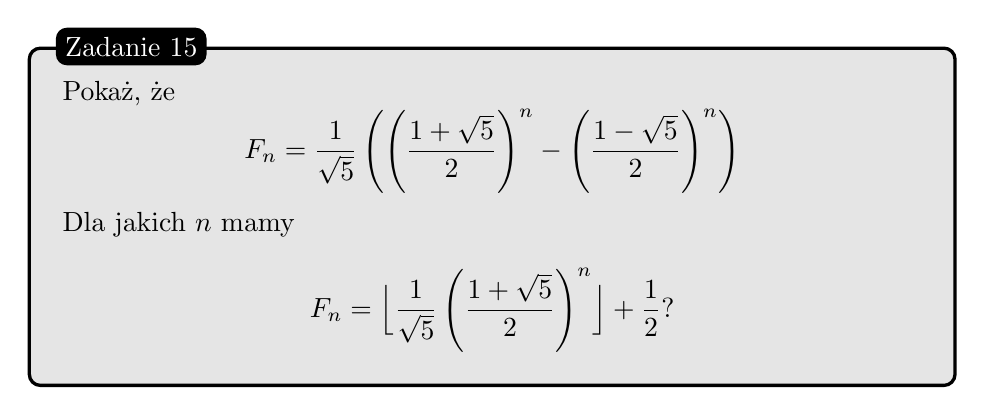
\begin{tikzpicture}
\node [draw={black}, fill=black!10, very thick, rectangle, rounded corners, inner sep=12pt, inner ysep=12pt] (box){%
    \begin{minipage}{.9\textwidth}

    Pokaż, że $$F_n = \frac{1}{\sqrt{5}} \left( \left( \frac{1 + \sqrt{5}}{2} \right)^n - \left( \frac{1 - \sqrt{5}}{2} \right)^n  \right)$$ Dla jakich $n$ mamy $$F_n = \Bigl\lfloor \frac{1}{\sqrt{5}} \left( \frac{1+\sqrt{5}}{2} \right)^n \Bigr\rfloor + \frac{1}{2} ?$$

    \end{minipage}
};
\node[fill={black}, text=white, rounded corners, right=10pt] at (box.north west) {Zadanie 15};
\end{tikzpicture}
\end{center}

\begin{thm}
$$F_n = \frac{1}{\sqrt{5}} \left( \left( \frac{1 + \sqrt{5}}{2} \right)^n - \left( \frac{1 - \sqrt{5}}{2} \right)^n  \right)$$
\end{thm}

\begin{proof}

Wiemy z algebry (albo dowodzimy indukcyjnie), że zachodzi równość :

$\begin{pmatrix} 1 & 1 \\ 1 & 0 \end{pmatrix}^n \cdot \begin{pmatrix} F_1 \\ F_0 \end{pmatrix} =  \begin{pmatrix} F_{n+1} \\ F_n \end{pmatrix} $

Diagonalizujemy macierz $\begin{pmatrix} 1 & 1 \\ 1 & 0 \end{pmatrix}$. Po długich i żmudnych rachunkach dostaniemy :

$$\begin{pmatrix} 1 & 1 \\ 1 & 0 \end{pmatrix} = \begin{pmatrix} \frac{1}{2} \left( 1 - \sqrt{5} \right) & \frac{1}{2} \left( 1 + \sqrt{5} \right) \\ 1 & 1 \end{pmatrix} \cdot \begin{pmatrix} \frac{1}{2} \left( 1 - \sqrt{5} \right) & 0 \\ 0 & \frac{1}{2} \left( 1 + \sqrt{5} \right) \end{pmatrix} \cdot \begin{pmatrix} \frac{-1}{\sqrt{5}} & \frac{5+\sqrt{5}}{10} \\ \frac{1}{\sqrt{5}} & \frac{5-\sqrt{5}}{10} \end{pmatrix}$$

Jak to zrobić?

\begin{itemize}

\item Obliczamy wielomian charakterystyczny macierzy. Wychodzi on $x^2 - x - 1$ i ma pierwiastki odpowiednio $x_1 = \frac{1+ \sqrt{5}}{2}$ i $x_2 = \frac{1 - \sqrt{5}}{2}$.

\item Dla każdej wartości własnej szukamy wektora własnego (bierzemy np. te które napisałem w macierzy).

\item Otrzymaną macierz odwracamy i zapisujemy całość w postaci $ABA^{-1}$, gdzie macierz $A$ to macierz której kolumnami są wektory własne, a macierz $B$ to macierz diagonalna z odpowiadającymi wartościami własnymi na przekątnej.
\end{itemize}

Teraz wystarczy tylko brutalnie obliczyć wynik.

$$\begin{pmatrix} F_{n+1} \\ F_n \end{pmatrix} = \begin{pmatrix} 1 & 1 \\ 1 & 0 \end{pmatrix}^n \cdot \begin{pmatrix} 1 \\ 0 \end{pmatrix} = \begin{pmatrix} \frac{1}{2} \left( 1 - \sqrt{5} \right) & \frac{1}{2} \left( 1 + \sqrt{5} \right) \\ 1 & 1 \end{pmatrix} \cdot \begin{pmatrix} \frac{1}{2} \left( 1 - \sqrt{5} \right)^n & 0 \\ 0 & \frac{1}{2} \left( 1 + \sqrt{5} \right)^n \end{pmatrix} \cdot \begin{pmatrix} \frac{-1}{\sqrt{5}} & \frac{5+\sqrt{5}}{10} \\ \frac{1}{\sqrt{5}} & \frac{5-\sqrt{5}}{10} \end{pmatrix} \cdot \begin{pmatrix} 1 \\ 0 \end{pmatrix} =  $$


$$
= \ldots = \begin{pmatrix} \frac{1}{\sqrt{5}} \left( \left( \frac{1 + \sqrt{5}}{2} \right)^{n+1} - \left( \frac{1 - \sqrt{5}}{2} \right)^{n+1}  \right)\\ \frac{1}{\sqrt{5}} \left( \left( \frac{1 + \sqrt{5}}{2} \right)^n - \left( \frac{1 - \sqrt{5}}{2} \right)^n  \right) \end{pmatrix}
$$

Stąd już wniosek o tym, że $F_n = \frac{1}{\sqrt{5}} \left( \left( \frac{1 + \sqrt{5}}{2} \right)^n - \left( \frac{1 - \sqrt{5}}{2} \right)^n  \right)$.

\end{proof}

\begin{thm}
Dla dowolnego $n \in \mathbb{N}$ zachodzi równość

$$F_n = \Bigl\lfloor \frac{1}{\sqrt{5}} \left( \frac{1+\sqrt{5}}{2} \right)^n \Bigr\rfloor + \frac{1}{2}$$

\end{thm}

\begin{proof}
Weźmy dowolne $n \in \mathbb{N}$.
Pokażmy, że zachodzi nierówność

$$F_n \leq \frac{1}{\sqrt{5}} \left( \frac{1+\sqrt{5}}{2} \right)^n + \frac{1}{2} < 1 + F_n$$

Następnie z definicji podłogi dostaniemy tezę.

$$
1 + F_n = 1+ \frac{1}{\sqrt{5}} \left( \left( \frac{1 + \sqrt{5}}{2} \right)^n - \left( \frac{1 - \sqrt{5}}{2} \right)^n  \right) > \frac{1}{\sqrt{5}} \left( \frac{1+\sqrt{5}}{2} \right)^n
$$

$$ 1 > \frac{1}{\sqrt{5}} \left( \frac{1-\sqrt{5}}{2} \right)^n$$

$$\sqrt{5} \cdot 2^n > \left(1-\sqrt{5}) \right)^n$$

Ostatnia linijka jest prawdą, ponieważ $1-\sqrt{5} \approx -1.24$. Została nam do pokazania tylko druga nierówność.

$$F_n = \frac{1}{\sqrt{5}} \left( \left( \frac{1 + \sqrt{5}}{2} \right)^n - \left( \frac{1 - \sqrt{5}}{2} \right)^n  \right)  \leq \frac{1}{\sqrt{5}} \left( \frac{1+\sqrt{5}}{2} \right)^n + \frac{1}{2} $$

Przekształcając powyższą nierónowść do postaci $-(1-\sqrt{5})^n \leq 2^{n-1} \cdot \sqrt{5}$, bo $-(1-\sqrt{5})^n \leq 2^n \leq 2^{n-1} \cdot \sqrt{5}$, co wiemy z poprzednich szacowań.
\end{proof}


%----------------------------------------------------------------------------------------

\end{document}